\section{Mutaciones puntuales de prote\'{i}nas} \label{pointmut}

Un problema que se presenta con cada vez mayor frecuencia desde que llegaron las tecnolog\'{i}as de 
ultrasecuenciaci\'{o}n es el de estimar el fenotipo molecular de un polimorfismo gen\'{e}tico, 
por ejemplo un SNP que cambia la secuencia de amino\'{a}cidos de una prote\'{i}na al provocar 
una sustituci\'{o}n no sin\'{o}nima (\italics{missense}). 
Esto es necesario porque hay muchos m\'{a}s genotipos que fenotipos observados, y porque cu\'{a}nto m\'{a}s se secuencia se hace
patente que los individuos de una especie son portadores de m\'{u}ltiples mutaciones de diferente naturaleza
\citep{Peterson2013}.

Esto se relaciona con los resultados de \citet{Chothia1986}, presentados en la secci\'{o}n \ref{3dcons}, que 
observaron que los efectos de las mutaciones sobre la estructura (y por tanto la funci\'{o}n) dependen en
parte de d\'{o}nde se produzcan. No tiene el mismo efecto cambiar un amino\'{a}cido enterrado que uno en un
\italics{loop}, o uno que coevoluciona con otro de un lazo vecino. Del mismo modo, una sustituci\'{o}n en el interior
de una h\'{e}lice no se puede comparar con la eliminaci\'{o}n de un residuo catal\'{i}tico \citep{Berrondo2011}
o de otro clave para interaccionar con otras prote\'{i}nas \citep{deJuan2013}. 
El muestreo a gran escala de \citet{Rocklin2017} estudi\'{o} la estabilidad de miles de miniprote\'{i}nas (hasta 50aa) sint\'{e}ticas 
y unas 500 naturales del PDB nos ha proporcionado los mejores datos hasta la fecha. En esencia lo que hacen es medir la estabilidad 
de miles de secuencias de amino\'{a}cidos expres\'{a}ndolas y exponi\'{e}ndolas a proteasas en levadura.
De esa manera estiman el efecto que tienen mutaciones individuales dependiendo de su contexto de estructura secundaria, 
ya sea una alfa-h\'{e}lice, una l\'{a}mina beta o un lazo o loop:

\begin{figure}
\begin{center} 
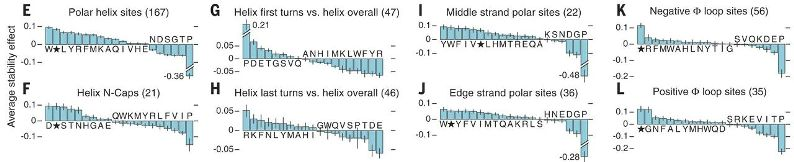
\includegraphics{stabilityTable}
\caption%[]
{
Efecto sobre la estabilidad de mutaciones en diferentes contextos estructurales. 
Los valores negativos, como los de la prolina en general, son desestabilizadores. 
Adaptada de \citet{Rocklin2017}. Copyright (2017) Science.
}
\label{fig:miniprotstab} %https://www.ncbi.nlm.nih.gov/pmc/articles/PMC5568797/
\end{center}
\end{figure}

\begin{figure}
\begin{center} 
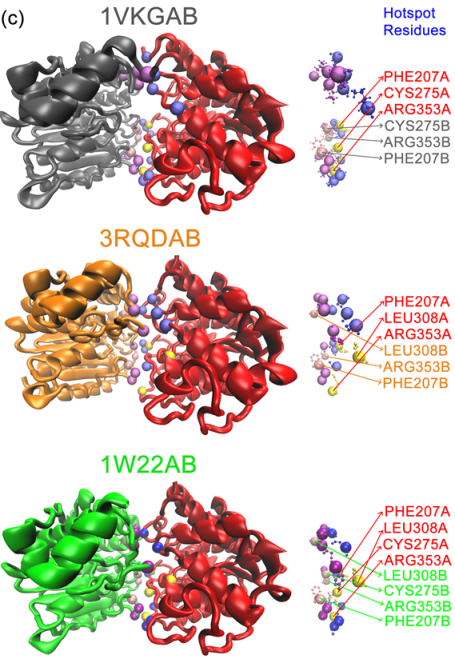
\includegraphics{ppi_interface}
\caption%[]
{
Grafo de la interfaz entre una histona-deacetilasa (en rojo) y tres parejas distintas.
Figura tomada de \citet{Cukuroglu2014} y reproducida con permiso de los autores.
}
\label{fig:ppi_interface}
\end{center}
\end{figure}

%\begin{figure}
%\begin{center} 
%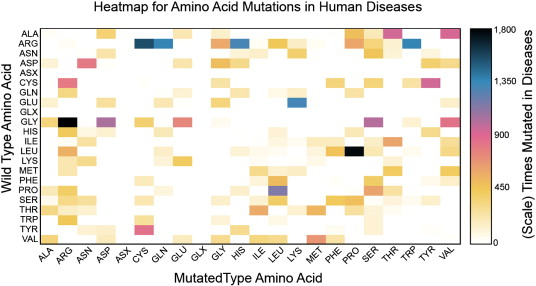
\includegraphics{human_mutations_heatmap}
%\caption%[]
%{
%Frecuencias de sustituci\'{o}n de amino\'{a}cidos en enfermedades humanas.
%Figura tomada de \citet{Peterson2013} y reproducida con permiso.}
%\label{fig:human_mutations_heatmap} %https://www.ncbi.nlm.nih.gov/pmc/articles/PMC3807015/
%\end{center}
%\end{figure}

Como se muestra en la figura \ref{fig:SNPpredictors}, hay una gran variedad de m\'{e}todos para la inferencia del fenotipo
molecular de mutaciones puntuales en prote\'{i}nas, y solamente algunos usan informaci\'{o}n estructural.
Probablemente el m\'{a}s universal de todos sea SIFT \citep{Kumar2009}, que usa como evidencia la
historia evolutiva de cada familia de prote\'{i}nas, que integra entre otras cosas determinantes estructurales
siempre y cuando haya suficientes secuencias hom\'{o}logas conocidas \citep{Saunders2002}. 
Sin embargo, como ocurre a menudo en biolog\'{i}a computacional, no es sencillo averiguar a partir de un
an\'{a}lisis de la literatura qu\'{e} m\'{e}todos son mejores. Hay que probarlos y escoger, y entre los
disponibles haya cada vez m\'{a}s alternativas que hacen un uso expl\'{i}cito de informaci\'{o}n
estructural, en concreto del contexto del residuo sustituido, como PolyPhen-2 \citep{Adzhubei2010},
SusPect \citep{Yates2014} o mCSM \citep{Pires2014}.

\begin{figure}
\begin{center} 
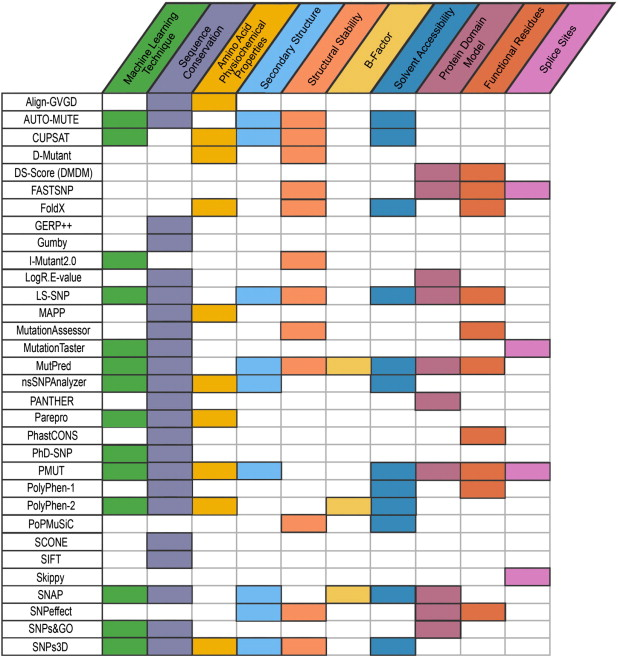
\includegraphics{SNPpredictors}
\caption%[]
{
Clasificaci\'{o}n de m\'{e}todos de inferencia de fenotipos de mutaciones no sin\'{o}nimas en base a los tipos de datos que emplean.
Figura tomada de \citet{Peterson2013} y reproducida con permiso.
}
\label{fig:SNPpredictors}
\end{center}
\end{figure}

\begin{figure}
\begin{center} 
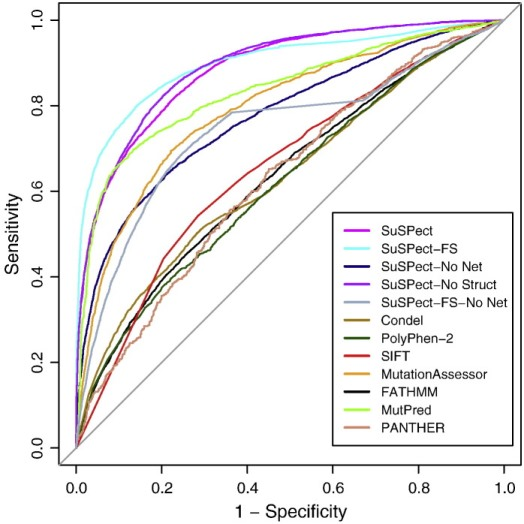
\includegraphics{SNP_performance}
\caption%[]
{
Comparaci\'{o}n del rendimiento de SusPect prediciendo mutaciones humanas delet\'{e}reas frente a otros predictores.
Figura tomada de \citep{Yates2014} y reproducida con permiso.
}
\label{fig:SNP_performance} %https://www.ncbi.nlm.nih.gov/pmc/articles/PMC4087249/
\end{center}
\end{figure}

Para explorar la predicci\'{o}n de fenotipos de mutaciones no sin\'{o}nimas planteo este ejercicio:
\begin{itemize}

\item Visita una base de datos de mutantes, como \htmladdnormallink{OMIM}{http://www.omim.org}, y elige una prote\'{i}na P (ejemplo: OPCML).

\item Obt\'{e}n la secuencia silvestre de amino\'{a}cidos S y al menos otra M con una mutaci\'{o}n delet\'{e}rea.

\item Construye un modelo comparativo de M y S.

\item Haz predicciones de fenotipo para S y M con ayuda, por ejemplo, de: \htmladdnormallink{SIFT}{http://sift.jcvi.org/}, 
\htmladdnormallink{PolyPhen-2}{http://genetics.bwh.harvard.edu/pph2/} y \htmladdnormallink{SusPect}{http://www.sbg.bio.ic.ac.uk/~suspect}.

\item Compara las predicciones obtenidas e interpr\'{e}talas a la luz de las estructuras modeladas. 
Qu\'{e} limitaciones del modelado comparativo afloran?

\end{itemize}
